\documentclass[14pt]{extbook}
\usepackage{multicol, enumerate, enumitem, hyperref, color, soul, setspace, parskip, fancyhdr} %General Packages
\usepackage{amssymb, amsthm, amsmath, bbm, latexsym, units, mathtools} %Math Packages
\everymath{\displaystyle} %All math in Display Style
% Packages with additional options
\usepackage[headsep=0.5cm,headheight=12pt, left=1 in,right= 1 in,top= 1 in,bottom= 1 in]{geometry}
\usepackage[usenames,dvipsnames]{xcolor}
\usepackage{dashrule}  % Package to use the command below to create lines between items
\newcommand{\litem}[1]{\item#1\hspace*{-1cm}\rule{\textwidth}{0.4pt}}
\pagestyle{fancy}
\lhead{Progress Quiz 4}
\chead{}
\rhead{Version A}
\lfoot{6286-1986}
\cfoot{}
\rfoot{Fall 2020}
\begin{document}

\begin{enumerate}
\litem{
Describe the end behavior of the polynomial below.\[ f(x) = -4(x - 3)^{4}(x + 3)^{5}(x - 6)^{2}(x + 6)^{2} \]\begin{enumerate}[label=\Alph*.]
\begin{multicols}{2}\item 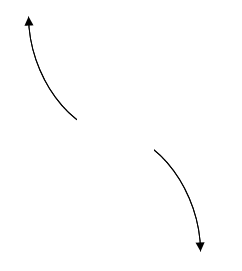
\includegraphics[width = 0.3\textwidth]{../Figures/polyEndBehaviorCopyAA.png}\item 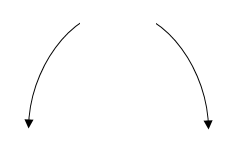
\includegraphics[width = 0.3\textwidth]{../Figures/polyEndBehaviorCopyBA.png}\item 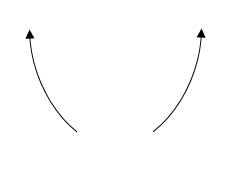
\includegraphics[width = 0.3\textwidth]{../Figures/polyEndBehaviorCopyCA.png}\item 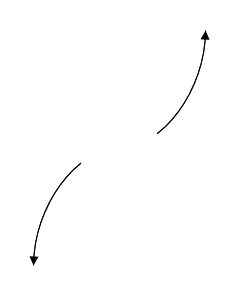
\includegraphics[width = 0.3\textwidth]{../Figures/polyEndBehaviorCopyDA.png}\end{multicols}\item None of the above.
\end{enumerate} }
\litem{
Construct the lowest-degree polynomial given the zeros below. Then, choose the intervals that contain the coefficients of the polynomial in the form $ax^3+bx^2+cx+d$.\[ -5, \frac{-3}{5}, \text{ and } \frac{6}{5} \]\begin{enumerate}[label=\Alph*.]
\item \( a \in [25, 34], b \in [106, 125], c \in [-95, -91], \text{ and } d \in [87, 95] \)
\item \( a \in [25, 34], b \in [-141, -137], c \in [52, 58], \text{ and } d \in [87, 95] \)
\item \( a \in [25, 34], b \in [-112, -103], c \in [-95, -91], \text{ and } d \in [87, 95] \)
\item \( a \in [25, 34], b \in [106, 125], c \in [-95, -91], \text{ and } d \in [-91, -88] \)
\item \( a \in [25, 34], b \in [-174, -169], c \in [239, 248], \text{ and } d \in [-91, -88] \)

\end{enumerate} }
\litem{
Construct the lowest-degree polynomial given the zeros below. Then, choose the intervals that contain the coefficients of the polynomial in the form $x^3+bx^2+cx+d$.\[ -2 - 3 i \text{ and } -4 \]\begin{enumerate}[label=\Alph*.]
\item \( b \in [-9, -7], c \in [28.54, 29.25], \text{ and } d \in [-53, -48] \)
\item \( b \in [4, 13], c \in [28.54, 29.25], \text{ and } d \in [47, 55] \)
\item \( b \in [-7, 3], c \in [5.19, 6.76], \text{ and } d \in [3, 9] \)
\item \( b \in [-7, 3], c \in [6.86, 8.71], \text{ and } d \in [10, 20] \)
\item \( \text{None of the above.} \)

\end{enumerate} }
\litem{
Describe the end behavior of the polynomial below.\[ f(x) = -5(x - 3)^{5}(x + 3)^{10}(x - 2)^{5}(x + 2)^{5} \]\begin{enumerate}[label=\Alph*.]
\begin{multicols}{2}\item 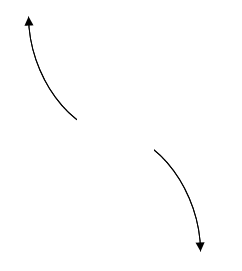
\includegraphics[width = 0.3\textwidth]{../Figures/polyEndBehaviorAA.png}\item 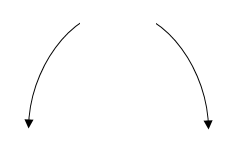
\includegraphics[width = 0.3\textwidth]{../Figures/polyEndBehaviorBA.png}\item 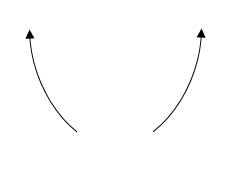
\includegraphics[width = 0.3\textwidth]{../Figures/polyEndBehaviorCA.png}\item 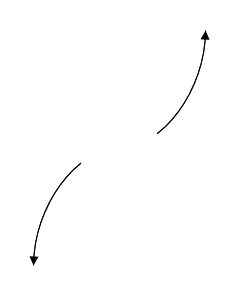
\includegraphics[width = 0.3\textwidth]{../Figures/polyEndBehaviorDA.png}\end{multicols}\item None of the above.
\end{enumerate} }
\litem{
Which of the following equations \textit{could} be of the graph presented below?
\begin{center}
    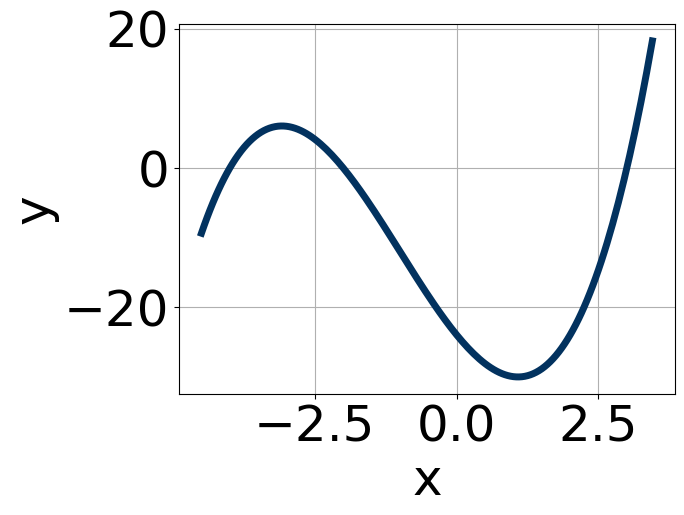
\includegraphics[width=0.5\textwidth]{../Figures/polyGraphToFunctionCopyA.png}
\end{center}
\begin{enumerate}[label=\Alph*.]
\item \( -15x^{7} (x + 3)^{8} (x + 2)^{5} \)
\item \( -20x^{4} (x + 3)^{8} (x + 2)^{9} \)
\item \( 4x^{9} (x + 3)^{6} (x + 2)^{9} \)
\item \( 18x^{7} (x + 3)^{6} (x + 2)^{4} \)
\item \( 13x^{7} (x + 3)^{5} (x + 2)^{10} \)

\end{enumerate} }
\litem{
Which of the following equations \textit{could} be of the graph presented below?
\begin{center}
    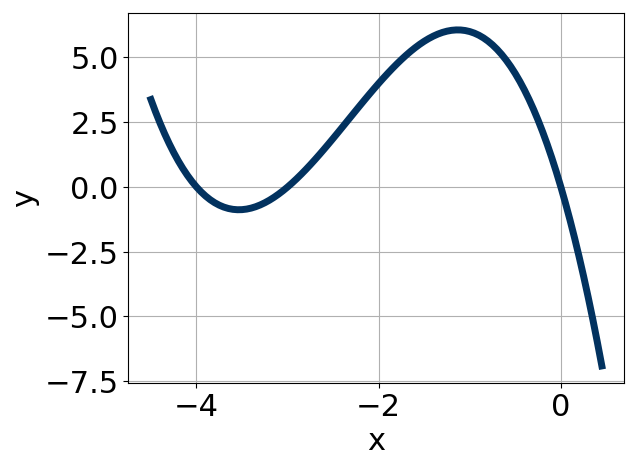
\includegraphics[width=0.5\textwidth]{../Figures/polyGraphToFunctionA.png}
\end{center}
\begin{enumerate}[label=\Alph*.]
\item \( 16x^{5} (x + 1)^{4} (x - 1)^{9} \)
\item \( 3x^{7} (x + 1)^{6} (x - 1)^{8} \)
\item \( -6x^{6} (x + 1)^{10} (x - 1)^{9} \)
\item \( 6x^{5} (x + 1)^{11} (x - 1)^{10} \)
\item \( -4x^{11} (x + 1)^{6} (x - 1)^{11} \)

\end{enumerate} }
\litem{
Construct the lowest-degree polynomial given the zeros below. Then, choose the intervals that contain the coefficients of the polynomial in the form $ax^3+bx^2+cx+d$.\[ -6, \frac{-1}{2}, \text{ and } \frac{-4}{3} \]\begin{enumerate}[label=\Alph*.]
\item \( a \in [0, 14], b \in [-27, -22], c \in [-65, -57], \text{ and } d \in [-24, -21] \)
\item \( a \in [0, 14], b \in [-51, -41], c \in [70, 76], \text{ and } d \in [-24, -21] \)
\item \( a \in [0, 14], b \in [39, 51], c \in [70, 76], \text{ and } d \in [-24, -21] \)
\item \( a \in [0, 14], b \in [39, 51], c \in [70, 76], \text{ and } d \in [19, 25] \)
\item \( a \in [0, 14], b \in [-36, -27], c \in [-37, -31], \text{ and } d \in [19, 25] \)

\end{enumerate} }
\litem{
Describe the zero behavior of the zero $x = 3$ of the polynomial below.\[ f(x) = -2(x + 3)^{7}(x - 3)^{8}(x - 2)^{9}(x + 2)^{11} \]\begin{enumerate}[label=\Alph*.]
\begin{multicols}{2}\item 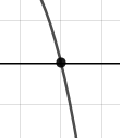
\includegraphics[width = 0.3\textwidth]{../Figures/polyZeroBehaviorCopyAA.png}\item 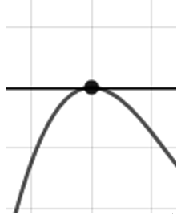
\includegraphics[width = 0.3\textwidth]{../Figures/polyZeroBehaviorCopyBA.png}\item 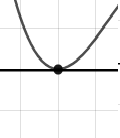
\includegraphics[width = 0.3\textwidth]{../Figures/polyZeroBehaviorCopyCA.png}\item 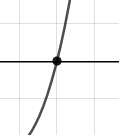
\includegraphics[width = 0.3\textwidth]{../Figures/polyZeroBehaviorCopyDA.png}\end{multicols}\item None of the above.
\end{enumerate} }
\litem{
Construct the lowest-degree polynomial given the zeros below. Then, choose the intervals that contain the coefficients of the polynomial in the form $x^3+bx^2+cx+d$.\[ -4 + 5 i \text{ and } 1 \]\begin{enumerate}[label=\Alph*.]
\item \( b \in [-1, 6], c \in [-10, -1], \text{ and } d \in [2, 7] \)
\item \( b \in [4, 11], c \in [32, 39], \text{ and } d \in [-43, -38] \)
\item \( b \in [-13, -3], c \in [32, 39], \text{ and } d \in [35, 44] \)
\item \( b \in [-1, 6], c \in [2, 4], \text{ and } d \in [-5, 4] \)
\item \( \text{None of the above.} \)

\end{enumerate} }
\litem{
Describe the zero behavior of the zero $x = -4$ of the polynomial below.\[ f(x) = -7(x + 4)^{6}(x - 4)^{9}(x - 7)^{5}(x + 7)^{7} \]\begin{enumerate}[label=\Alph*.]
\begin{multicols}{2}\item 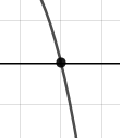
\includegraphics[width = 0.3\textwidth]{../Figures/polyZeroBehaviorAA.png}\item 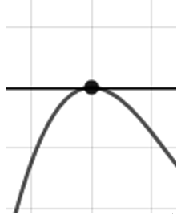
\includegraphics[width = 0.3\textwidth]{../Figures/polyZeroBehaviorBA.png}\item 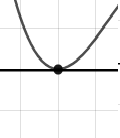
\includegraphics[width = 0.3\textwidth]{../Figures/polyZeroBehaviorCA.png}\item 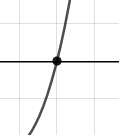
\includegraphics[width = 0.3\textwidth]{../Figures/polyZeroBehaviorDA.png}\end{multicols}\item None of the above.
\end{enumerate} }
\end{enumerate}

\end{document}